The expected number of signal and background events for an integrated 
luminosity of 1\ifb{} after applying the $\WW$ like selection are reported in 
Tab.~\ref{tab:wwselection0}(0-jet), Tab.~\ref{tab:wwselection1}(1-jet), 
Tab.~\ref{tab:wwselection2}(2-jet). The selection includes that none of the 
jets are top-tagged. In addition, the angle between the dilepton 
system and the jet in the transverse plane must be smaller than 165 dg. in 
the $ee/\mu\mu$ final states for the 1-jet bin. All simulated processes 
are reweighted to match the number of reconstructed vertexes in data, as 
explained in Appendix~\ref{app:vertex_reweight}, and the $gg \to H \to WW$ 
simulated events are reweighted to match the Higgs $\pt$ at NNLO, as explained 
in Section~\ref{sec:datasets}. The corresponding $\Delta\phi$, 
di-lepton mass, di-lepton $p_T$, $m_T$ and projected $\met$ distributions are 
shown in Figs.~\ref{fig:dPhi_jets0}-\ref{fig:pmet_jets0}(0-jet) 
and Figs.~\ref{fig:dPhi_jets1}-\ref{fig:pmet_jets1}(1-jet).

\begin{table}[!ht]
  \begin{center}
 {\scriptsize
  \begin{tabular} {|c|c|c|c|c|c|c|c|c|c|c|}
\hline
  & $\dy+WZ+ZZ$ & $\ttbar$ & $tW$ & $\Wjets$ & non-resonant $VV$ & $gg \to WW$ & $qq \to WW$ & H$_{130}$ &   H$_{160}$ \\
  \hline
  \hline
  $\M\M$   &  4.6$\pm$1.1 &  5.9$\pm$1.1 &  2.7$\pm$0.3 &   7.2$\pm$4.5 &  2.0$\pm$0.1 &  4.2$\pm$0.1 & 76.3$\pm$0.8 & 10.0$\pm$0.2 & 31.0$\pm$0.6\\
  $\E\E$   &  5.0$\pm$2.1 &  3.2$\pm$0.8 &  2.4$\pm$0.3 &  16.3$\pm$6.9 &  1.2$\pm$0.1 &  3.0$\pm$0.1 & 48.8$\pm$0.6 &  5.8$\pm$0.1 & 19.7$\pm$0.4\\
  $\E\M$   &  0.2$\pm$0.1 &  9.0$\pm$1.3 &  3.9$\pm$0.3 &  23.4$\pm$7.8 &  3.4$\pm$0.1 &  5.6$\pm$0.1 &117.8$\pm$1.0 & 12.3$\pm$0.2 & 30.9$\pm$0.6\\
  $\M\E$   &  3.9$\pm$2.2 &  8.4$\pm$1.2 &  3.8$\pm$0.3 &  26.9$\pm$9.2 &  2.6$\pm$0.1 &  5.2$\pm$0.1 &107.4$\pm$0.9 & 10.1$\pm$0.2 & 28.8$\pm$0.6\\
 \hline
       all & 13.7$\pm$3.3 & 26.6$\pm$2.2 & 12.7$\pm$0.6 &  73.9$\pm$14.7&  9.2$\pm$0.3 & 18.0$\pm$0.2 &350.3$\pm$1.7 & 38.2$\pm$0.8 &110.4$\pm$2.2\\
 \hline
  \end{tabular}
  }
  \caption{Expected number of signal and background events for an 
  integrated luminosity of 1\ifb{} after applying the \ww\ 
  0-jet selection requirements. Monte Carlo statistical 
  uncertainties are included.}
   \label{tab:wwselection0}
  \end{center}
\end{table}

\begin{table}[!ht]
  \begin{center}
 {\scriptsize
  \begin{tabular} {|c|c|c|c|c|c|c|c|c|c|c|}
\hline
  & $\dy+WZ+ZZ$ & $\ttbar$ & $tW$ & $\Wjets$ & non-resonant $VV$ & $gg \to WW$ & $qq \to WW$ & H$_{130}$ &   H$_{160}$ \\
  \hline
  \hline
  $\M\M$   &  6.2$\pm$2.2 & 15.0$\pm$1.7 &  4.4$\pm$0.4 &   3.0$\pm$3.0 &  0.8$\pm$0.1 &  1.2$\pm$0.1 & 20.8$\pm$0.4 &  3.0$\pm$0.7 & 11.3$\pm$0.2 \\
  $\E\E$   &  3.9$\pm$1.6 & 10.6$\pm$1.4 &  2.7$\pm$0.3 &   5.2$\pm$4.0 &  1.1$\pm$0.1 &  0.8$\pm$0.1 & 13.2$\pm$0.3 &  2.0$\pm$0.5 &  7.4$\pm$0.1 \\
  $\E\M$   &  5.5$\pm$2.3 & 27.2$\pm$2.2 &  7.5$\pm$0.5 &   6.1$\pm$4.3 &  3.2$\pm$0.1 &  2.0$\pm$0.1 & 34.3$\pm$0.5 &  4.6$\pm$0.9 & 13.6$\pm$0.3 \\
  $\M\E$   &  1.6$\pm$1.0 & 23.3$\pm$2.1 &  6.3$\pm$0.4 &   2.6$\pm$2.2 &  2.1$\pm$0.1 &  1.6$\pm$0.1 & 31.3$\pm$0.5 &  3.9$\pm$0.8 & 12.7$\pm$0.3 \\
 \hline
       all & 17.2$\pm$3.6 & 76.1$\pm$3.7 & 21.0$\pm$0.8 &  16.9$\pm$7.0 &  7.2$\pm$0.3 &  5.6$\pm$0.1 & 99.7$\pm$0.9 & 13.4$\pm$0.3 & 45.0$\pm$0.9 \\
 \hline
  \end{tabular}
  }
  \caption{Expected number of signal and background events for an 
  integrated luminosity of 1\ifb{} after applying the \ww\ 
  1-jet selection requirements. Monte Carlo statistical 
  uncertainties are included.}
   \label{tab:wwselection1}
  \end{center}
\end{table}

\begin{table}[!ht]
  \begin{center}
 {\scriptsize
  \begin{tabular} {|c|c|c|c|c|c|c|c|c|c|c|}
\hline
  & $\dy+WZ+ZZ$ & $\ttbar$ & $tW$ & $\Wjets$ & non-resonant $VV$ & $gg \to WW$ & $qq \to WW$ & H$_{130}$ &   H$_{160}$ \\
  \hline
  \hline
  $\M\M$   & 11.7$\pm$4.0 & 18.2$\pm$1.8 &  1.6$\pm$0.2 &   0.0$\pm$0.0 &  0.2$\pm$0.1 &  0.2$\pm$0.1 &  4.5$\pm$0.2 &  1.2$\pm$0.1 &  4.2$\pm$0.1 \\
  $\E\E$   &  6.6$\pm$2.6 & 13.4$\pm$1.6 &  1.1$\pm$0.2 &   0.0$\pm$0.0 &  0.3$\pm$0.1 &  0.1$\pm$0.1 &  3.1$\pm$0.2 &  0.7$\pm$0.1 &  2.6$\pm$0.1 \\
  $\E\M$   &  2.9$\pm$1.9 & 30.4$\pm$2.4 &  3.3$\pm$0.3 &   0.0$\pm$0.0 &  0.6$\pm$0.1 &  0.3$\pm$0.1 &  7.5$\pm$0.2 &  1.5$\pm$0.1 &  4.5$\pm$0.1 \\
  $\M\E$   &  1.8$\pm$1.2 & 24.4$\pm$2.1 &  2.0$\pm$0.2 &   3.8$\pm$3.8 &  0.4$\pm$0.1 &  0.3$\pm$0.1 &  6.1$\pm$0.2 &  1.3$\pm$0.1 &  3.9$\pm$0.1 \\
 \hline
       all & 23.1$\pm$5.3 & 86.4$\pm$4.0 &  8.0$\pm$0.5 &   3.8$\pm$3.8 &  1.5$\pm$0.1 &  1.0$\pm$0.1 & 21.2$\pm$0.4 &  4.7$\pm$0.2 & 15.2$\pm$0.2 \\
 \hline
  \end{tabular}
  }
  \caption{Expected number of signal and background events for an 
  integrated luminosity of 1\ifb{} after applying the \ww\ 
  2-jet selection requirements. Monte Carlo statistical 
  uncertainties are included.}
   \label{tab:wwselection2}
  \end{center}
\end{table}


\begin{figure}[!hbtp]
\centering
\subfigure[]{
\centering
\label{subfig:dPhi_hm120_jets0}
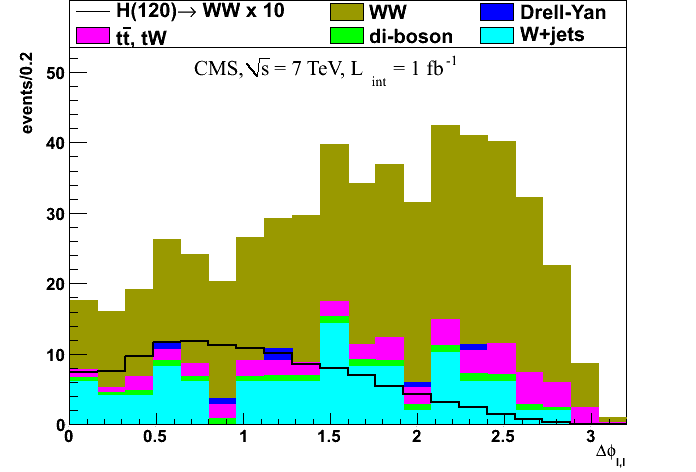
\includegraphics[width=.32\textwidth]{figures/dPhi_hm120_jets0.png}}
\subfigure[]{
\centering
\label{subfig:dPhi_hm160_jets0}
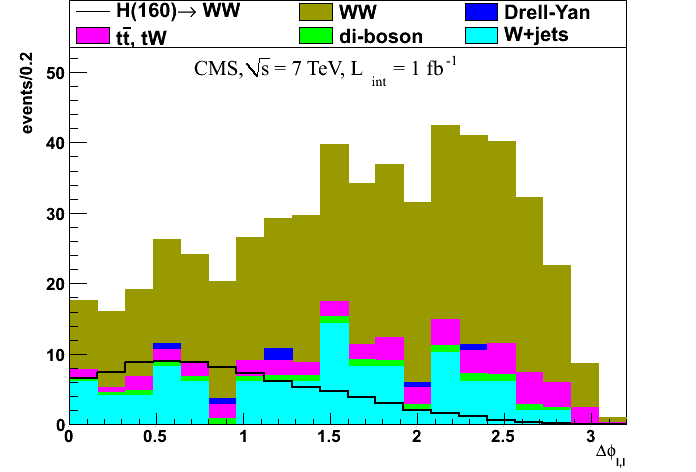
\includegraphics[width=.32\textwidth]{figures/dPhi_hm160_jets0.png}}
\subfigure[]{
\centering
\label{subfig:dPhi_hm250_jets0}
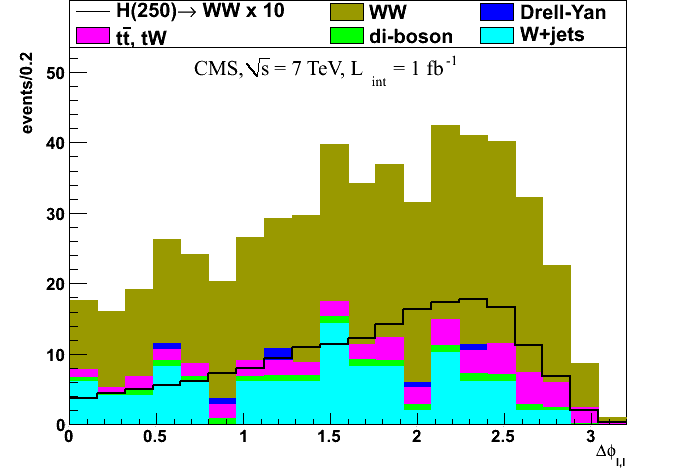
\includegraphics[width=.32\textwidth]{figures/dPhi_hm250_jets0.png}}\\
\caption{Lepton $\Delta\phi$ distribution after \WW\ selection for $m_H$=120 $\GeVcc$ \subref{subfig:dPhi_hm120_jets0}, 
$m_H$=160 $\GeVcc$ \subref{subfig:dPhi_hm160_jets0} and $m_H$=250 $\GeVcc$ \subref{subfig:dPhi_hm250_jets0} in the 0-jet bin.}
\label{fig:dPhi_jets0}
\end{figure}

\begin{figure}[!hbtp]
\centering
\subfigure[]{
\centering
\label{subfig:dilepmass_hm120_jets0}
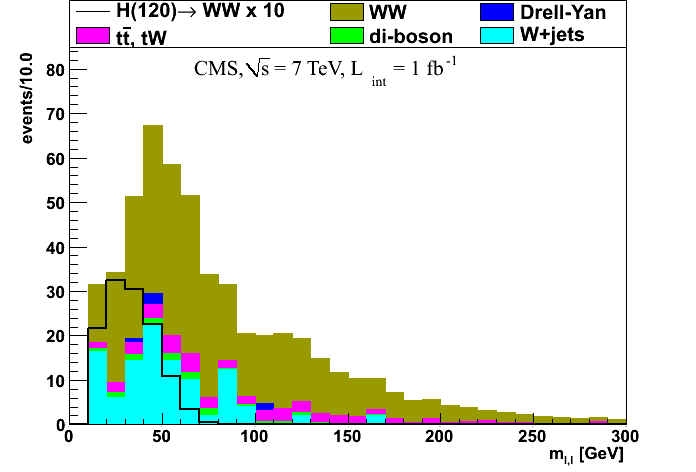
\includegraphics[width=.32\textwidth]{figures/dilepmass_hm120_jets0.png}}
\subfigure[]{
\centering
\label{subfig:dilepmass_hm160_jets0}
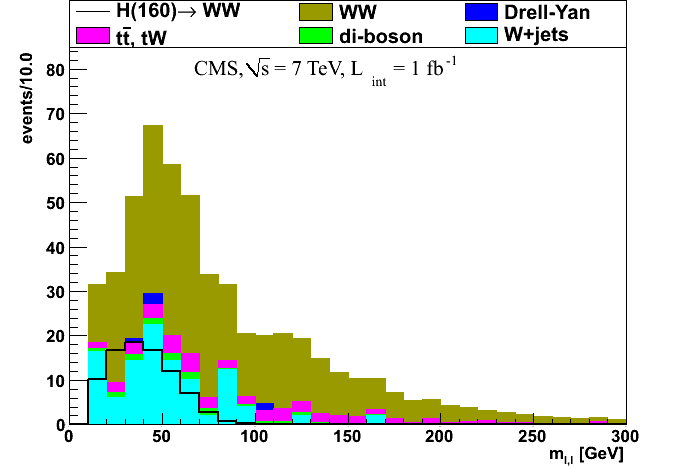
\includegraphics[width=.32\textwidth]{figures/dilepmass_hm160_jets0.png}}
\subfigure[]{
\centering
\label{subfig:dilepmass_hm250_jets0}
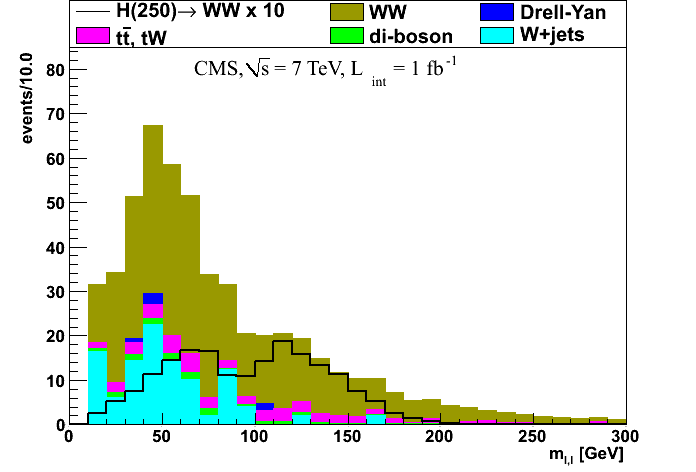
\includegraphics[width=.32\textwidth]{figures/dilepmass_hm250_jets0.png}}\\
\caption{Di-lepton mass distribution after \WW\ selection for $m_H$=120 $\GeVcc$ \subref{subfig:dilepmass_hm120_jets0}, 
$m_H$=160 $\GeVcc$ \subref{subfig:dilepmass_hm160_jets0} and $m_H$=250 $\GeVcc$ \subref{subfig:dilepmass_hm250_jets0} in the 0-jet bin.}
\label{fig:dilepmass_jets0}
\end{figure}

\begin{figure}[!hbtp]
\centering
\subfigure[]{
\centering
\label{subfig:dileppt_hm120_jets0}
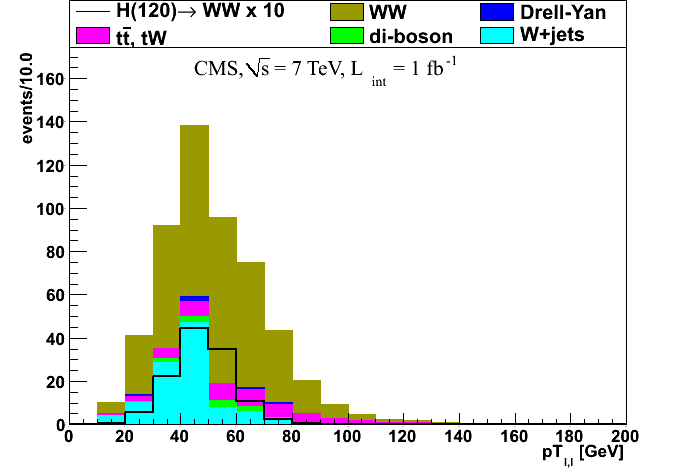
\includegraphics[width=.32\textwidth]{figures/dileppt_hm120_jets0.png}}
\subfigure[]{
\centering
\label{subfig:dileppt_hm160_jets0}
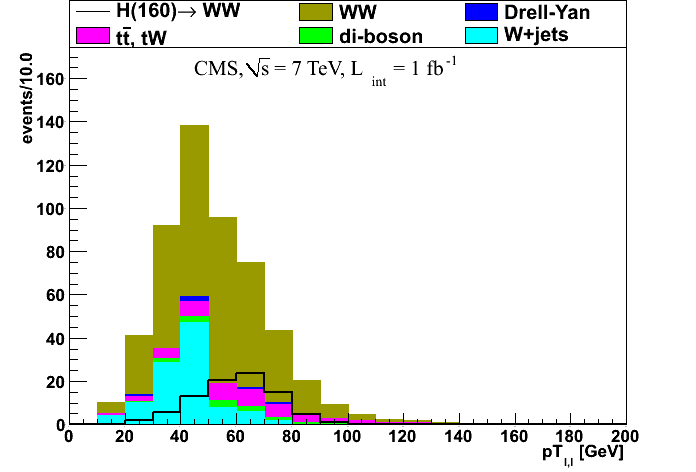
\includegraphics[width=.32\textwidth]{figures/dileppt_hm160_jets0.png}}
\subfigure[]{
\centering
\label{subfig:dileppt_hm250_jets0}
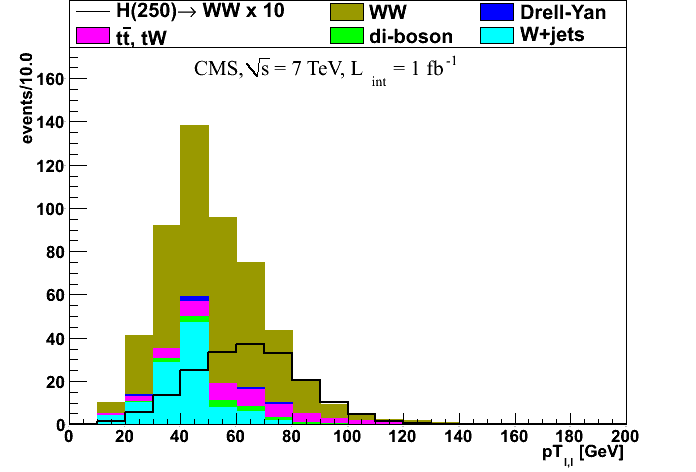
\includegraphics[width=.32\textwidth]{figures/dileppt_hm250_jets0.png}}\\
\caption{Di-lepton $p_T$ distribution after \WW\ selection for $m_H$=120 $\GeVcc$ \subref{subfig:dileppt_hm120_jets0}, 
$m_H$=160 $\GeVcc$ \subref{subfig:dileppt_hm160_jets0} and $m_H$=250 $\GeVcc$ \subref{subfig:dileppt_hm250_jets0} in the 0-jet bin.}
\label{fig:dileppt_jets0}
\end{figure}

\begin{figure}[!hbtp]
\centering
\subfigure[]{
\centering
\label{subfig:mt_hm120_jets0}
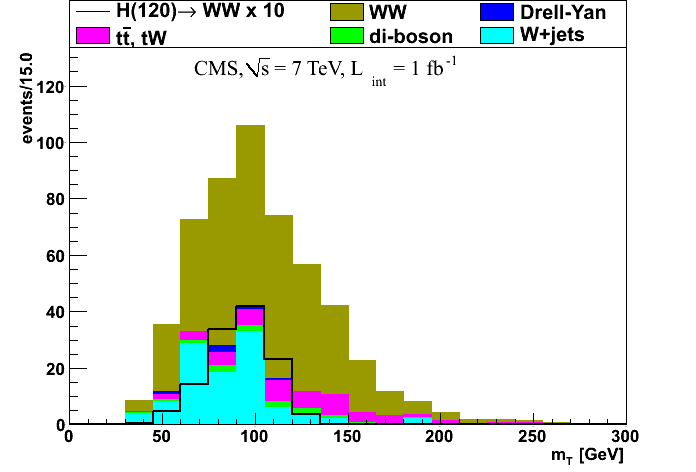
\includegraphics[width=.32\textwidth]{figures/mt_hm120_jets0.png}}
\subfigure[]{
\centering
\label{subfig:mt_hm160_jets0}
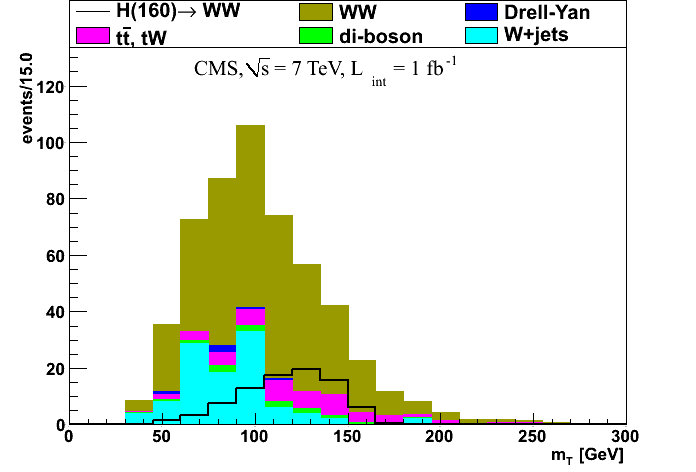
\includegraphics[width=.32\textwidth]{figures/mt_hm160_jets0.png}}
\subfigure[]{
\centering
\label{subfig:mt_hm250_jets0}
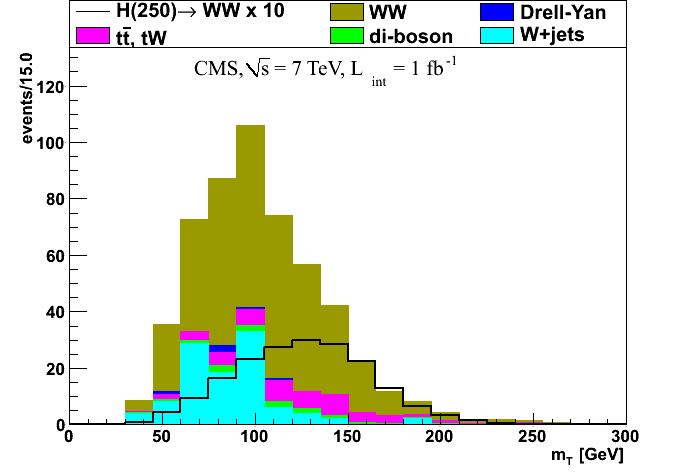
\includegraphics[width=.32\textwidth]{figures/mt_hm250_jets0.png}}\\
\caption{$m_T$ distribution after \WW\ selection for $m_H$=120 $\GeVcc$ \subref{subfig:mt_hm120_jets0}, 
$m_H$=160 $\GeVcc$ \subref{subfig:mt_hm160_jets0} and $m_H$=250 $\GeVcc$ \subref{subfig:mt_hm250_jets0} in the 0-jet bin.}
\label{fig:mt_jets0}
\end{figure}

\begin{figure}[!hbtp]
\centering
\subfigure[]{
\centering
\label{subfig:pmet_hm120_jets0}
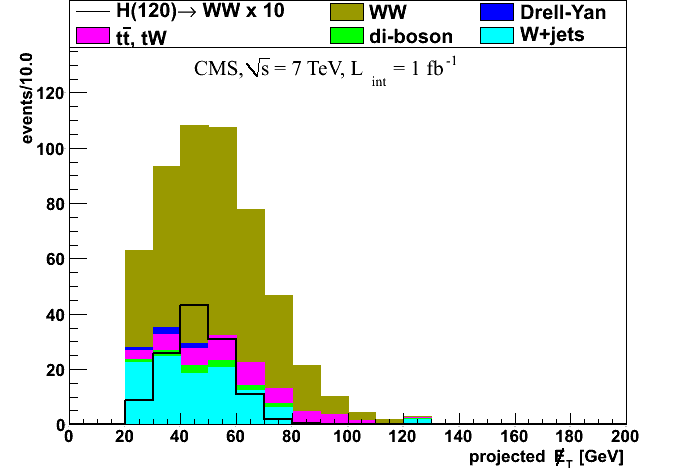
\includegraphics[width=.32\textwidth]{figures/pmet_hm120_jets0.png}}
\subfigure[]{
\centering
\label{subfig:pmet_hm160_jets0}
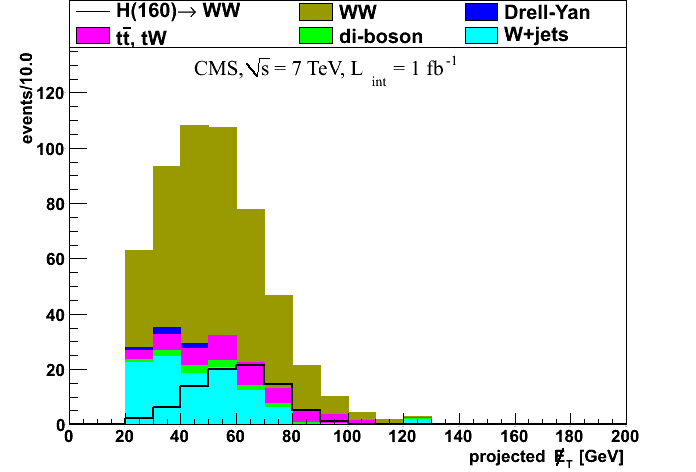
\includegraphics[width=.32\textwidth]{figures/pmet_hm160_jets0.png}}
\subfigure[]{
\centering
\label{subfig:pmet_hm250_jets0}
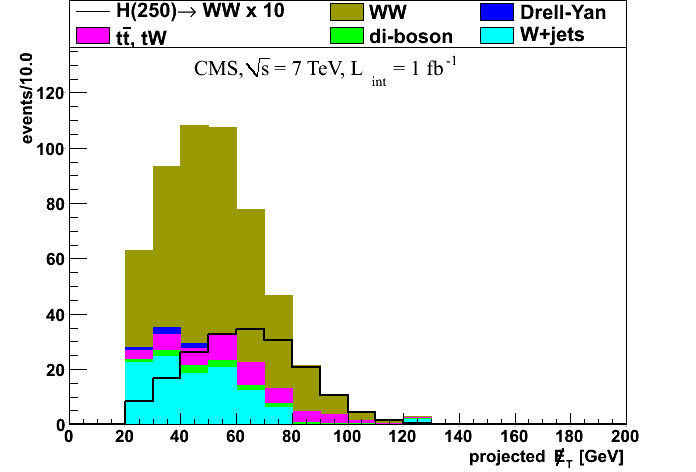
\includegraphics[width=.32\textwidth]{figures/pmet_hm250_jets0.png}}\\
\caption{Projected $\met$ distribution after \WW\ selection for $m_H$=120 $\GeVcc$ \subref{subfig:pmet_hm120_jets0}, 
$m_H$=160 $\GeVcc$ \subref{subfig:pmet_hm160_jets0} and $m_H$=250 $\GeVcc$ \subref{subfig:pmet_hm250_jets0} in the 0-jet bin.}
\label{fig:pmet_jets0}
\end{figure}








\begin{figure}[!hbtp]
\centering
\subfigure[]{
\centering
\label{subfig:dPhi_hm120_jets1}
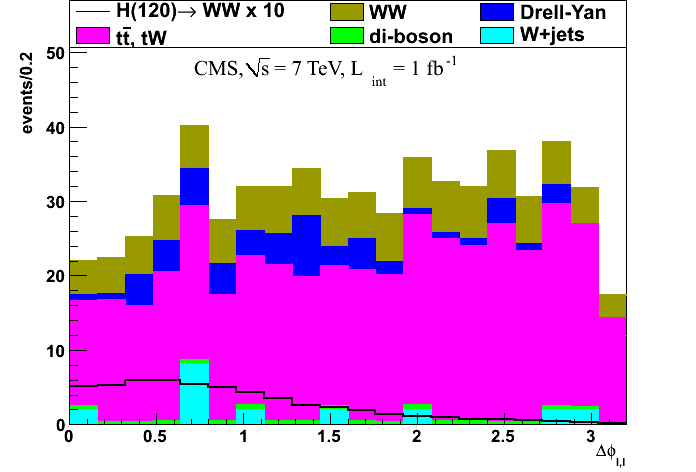
\includegraphics[width=.32\textwidth]{figures/dPhi_hm120_jets1.png}}
\subfigure[]{
\centering
\label{subfig:dPhi_hm160_jets1}
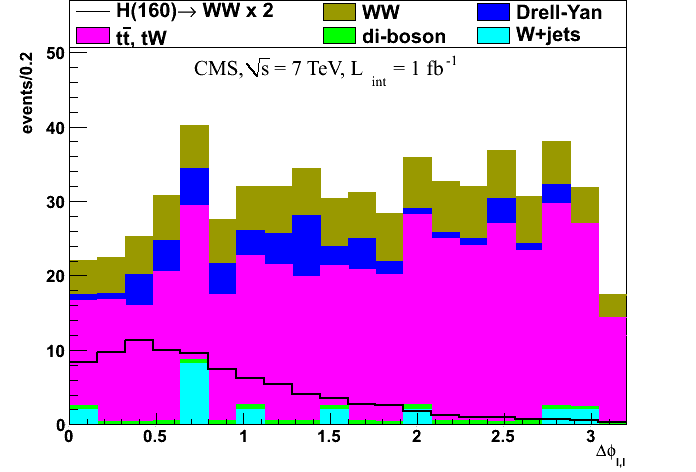
\includegraphics[width=.32\textwidth]{figures/dPhi_hm160_jets1.png}}
\subfigure[]{
\centering
\label{subfig:dPhi_hm250_jets1}
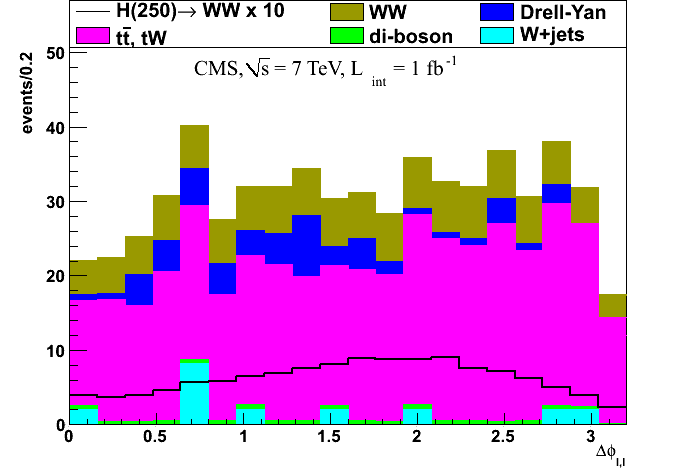
\includegraphics[width=.32\textwidth]{figures/dPhi_hm250_jets1.png}}\\
\caption{Lepton $\Delta\phi$ distribution after \WW\ selection for $m_H$=120 $\GeVcc$ \subref{subfig:dPhi_hm120_jets1}, 
$m_H$=160 $\GeVcc$ \subref{subfig:dPhi_hm160_jets1} and $m_H$=250 $\GeVcc$ \subref{subfig:dPhi_hm250_jets1} in the 1-jet bin.}
\label{fig:dPhi_jets1}
\end{figure}

\begin{figure}[!hbtp]
\centering
\subfigure[]{
\centering
\label{subfig:dilepmass_hm120_jets1}
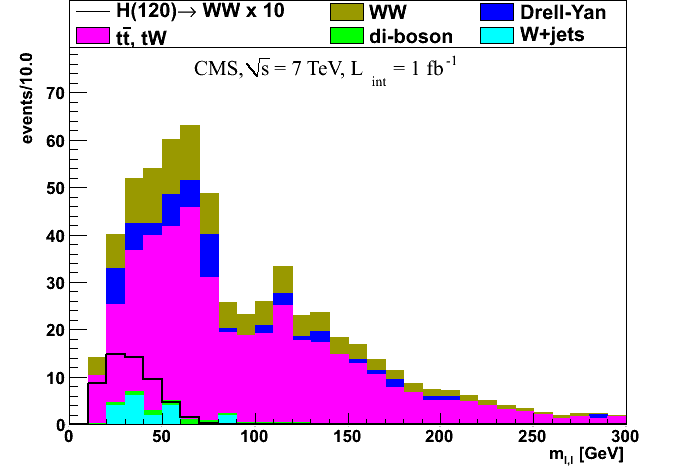
\includegraphics[width=.32\textwidth]{figures/dilepmass_hm120_jets1.png}}
\subfigure[]{
\centering
\label{subfig:dilepmass_hm160_jets1}
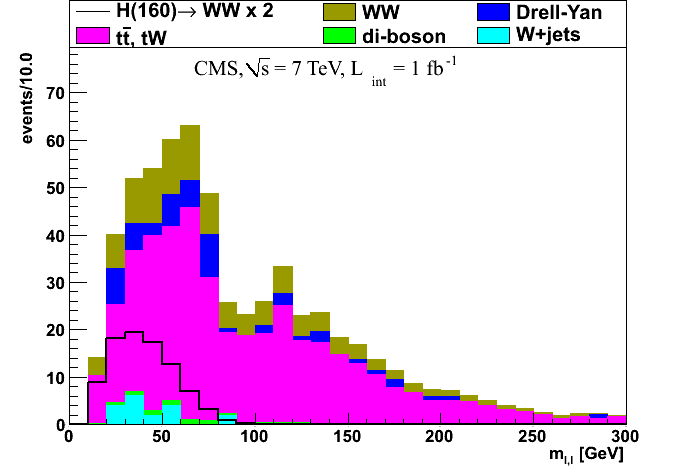
\includegraphics[width=.32\textwidth]{figures/dilepmass_hm160_jets1.png}}
\subfigure[]{
\centering
\label{subfig:dilepmass_hm250_jets1}
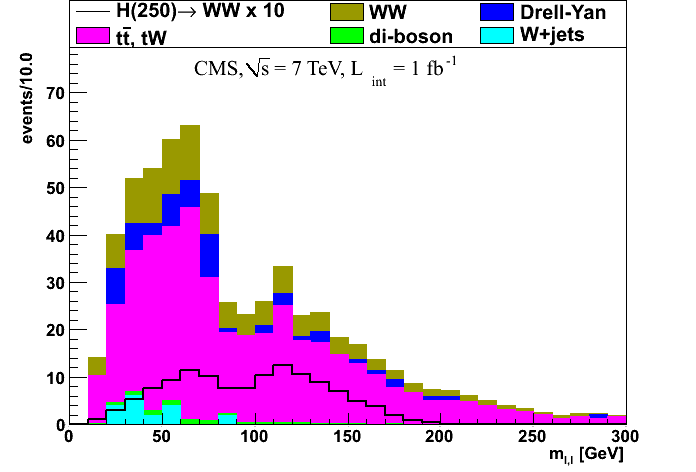
\includegraphics[width=.32\textwidth]{figures/dilepmass_hm250_jets1.png}}\\
\caption{Di-lepton mass distribution after \WW\ selection for $m_H$=120 $\GeVcc$ \subref{subfig:dilepmass_hm120_jets1}, 
$m_H$=160 $\GeVcc$ \subref{subfig:dilepmass_hm160_jets1} and $m_H$=250 $\GeVcc$ \subref{subfig:dilepmass_hm250_jets1} in the 1-jet bin.}
\label{fig:dilepmass_jets1}
\end{figure}

\begin{figure}[!hbtp]
\centering
\subfigure[]{
\centering
\label{subfig:dileppt_hm120_jets1}
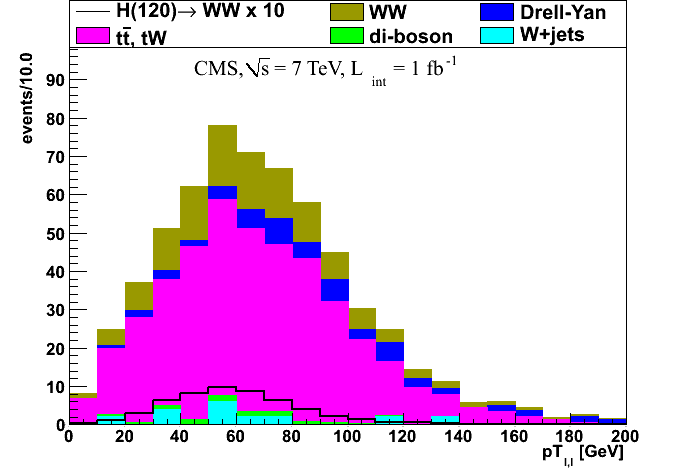
\includegraphics[width=.32\textwidth]{figures/dileppt_hm120_jets1.png}}
\subfigure[]{
\centering
\label{subfig:dileppt_hm160_jets1}
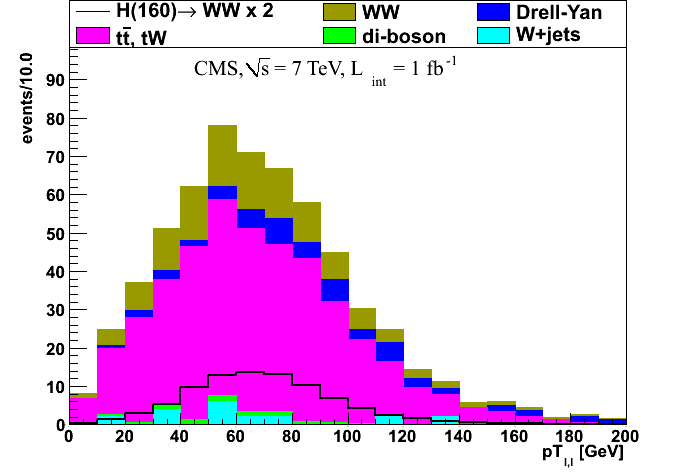
\includegraphics[width=.32\textwidth]{figures/dileppt_hm160_jets1.png}}
\subfigure[]{
\centering
\label{subfig:dileppt_hm250_jets1}
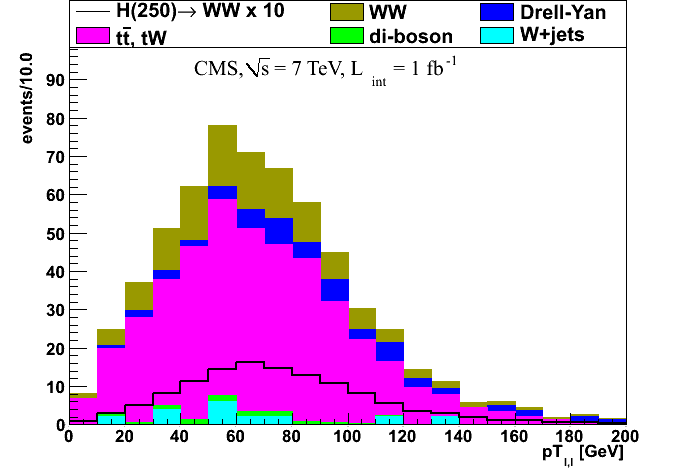
\includegraphics[width=.32\textwidth]{figures/dileppt_hm250_jets1.png}}\\
\caption{Di-lepton $p_T$ distribution after \WW\ selection for $m_H$=120 $\GeVcc$ \subref{subfig:dileppt_hm120_jets1}, 
$m_H$=160 $\GeVcc$ \subref{subfig:dileppt_hm160_jets1} and $m_H$=250 $\GeVcc$ \subref{subfig:dileppt_hm250_jets1} in the 1-jet bin.}
\label{fig:dileppt_jets1}
\end{figure}

\begin{figure}[!hbtp]
\centering
\subfigure[]{
\centering
\label{subfig:mt_hm120_jets1}
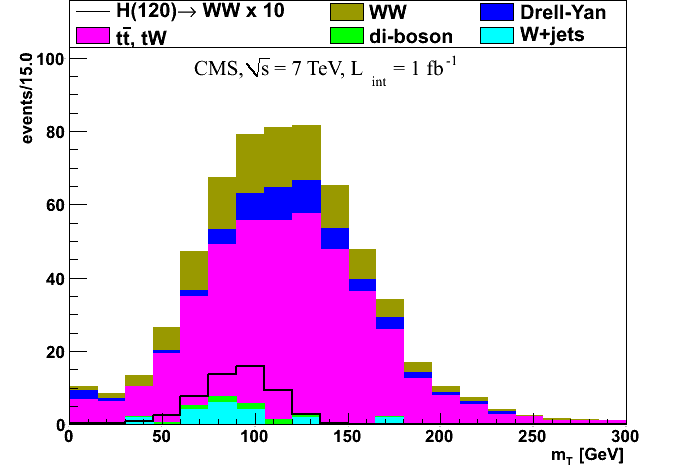
\includegraphics[width=.32\textwidth]{figures/mt_hm120_jets1.png}}
\subfigure[]{
\centering
\label{subfig:mt_hm160_jets1}
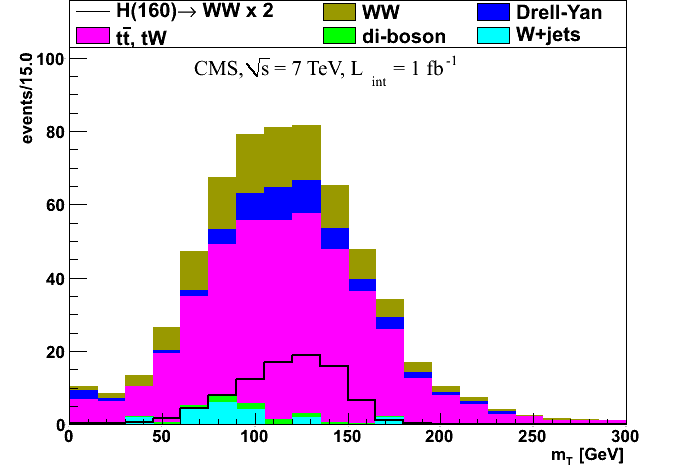
\includegraphics[width=.32\textwidth]{figures/mt_hm160_jets1.png}}
\subfigure[]{
\centering
\label{subfig:mt_hm250_jets1}
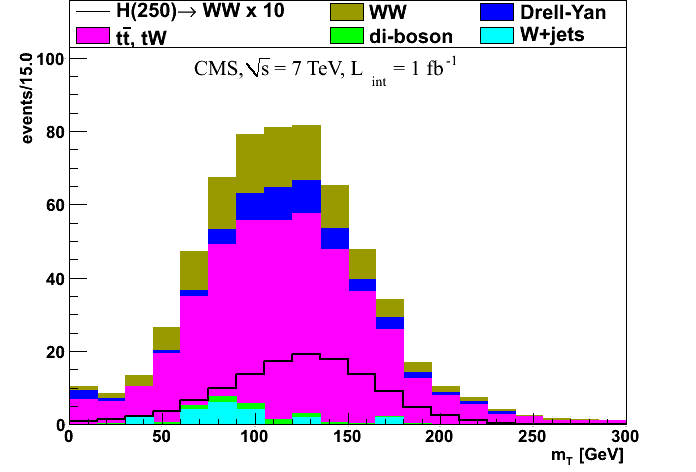
\includegraphics[width=.32\textwidth]{figures/mt_hm250_jets1.png}}\\
\caption{$m_T$ distribution after \WW\ selection for $m_H$=120 $\GeVcc$ \subref{subfig:mt_hm120_jets1}, 
$m_H$=160 $\GeVcc$ \subref{subfig:mt_hm160_jets1} and $m_H$=250 $\GeVcc$ \subref{subfig:mt_hm250_jets1} in the 1-jet bin.}
\label{fig:mt_jets1}
\end{figure}

\begin{figure}[!hbtp]
\centering
\subfigure[]{
\centering
\label{subfig:pmet_hm120_jets1}
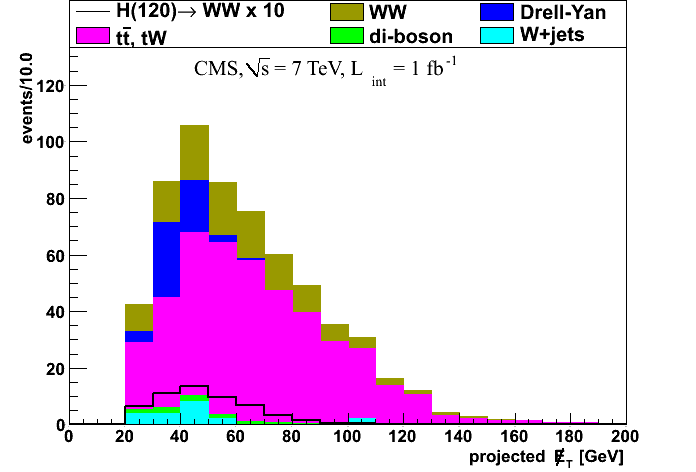
\includegraphics[width=.32\textwidth]{figures/pmet_hm120_jets1.png}}
\subfigure[]{
\centering
\label{subfig:pmet_hm160_jets1}
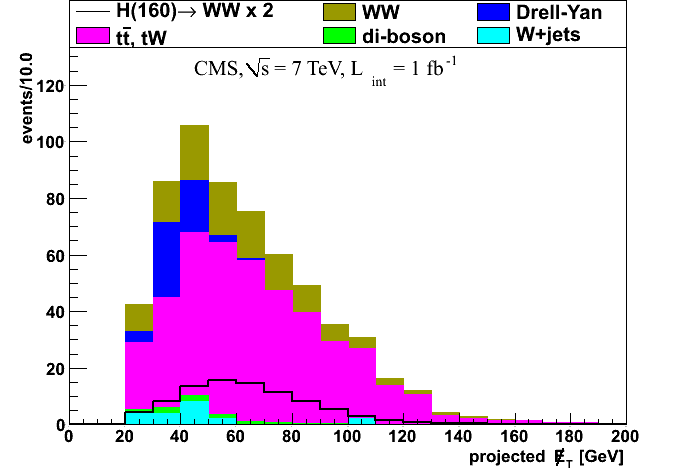
\includegraphics[width=.32\textwidth]{figures/pmet_hm160_jets1.png}}
\subfigure[]{
\centering
\label{subfig:pmet_hm250_jets1}
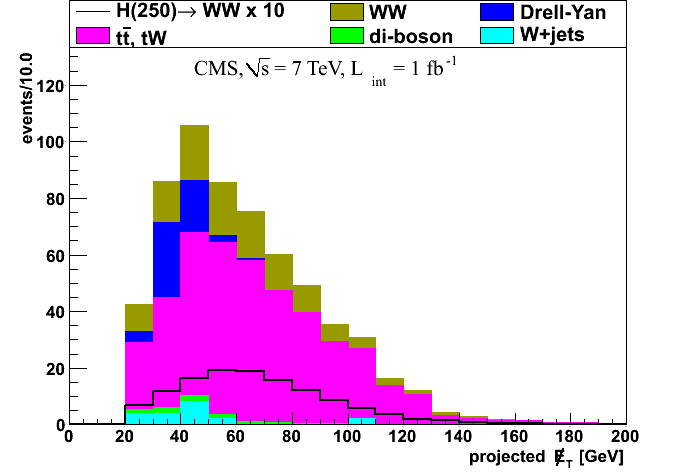
\includegraphics[width=.32\textwidth]{figures/pmet_hm250_jets1.png}}\\
\caption{Projected $\met$ distribution after \WW\ selection for $m_H$=120 $\GeVcc$ \subref{subfig:pmet_hm120_jets1}, 
$m_H$=160 $\GeVcc$ \subref{subfig:pmet_hm160_jets1} and $m_H$=250 $\GeVcc$ \subref{subfig:pmet_hm250_jets1} in the 1-jet bin.}
\label{fig:pmet_jets1}
\end{figure}
